\begin{frame}{Antecedentes}    
    \begin{figure}
        \centering
        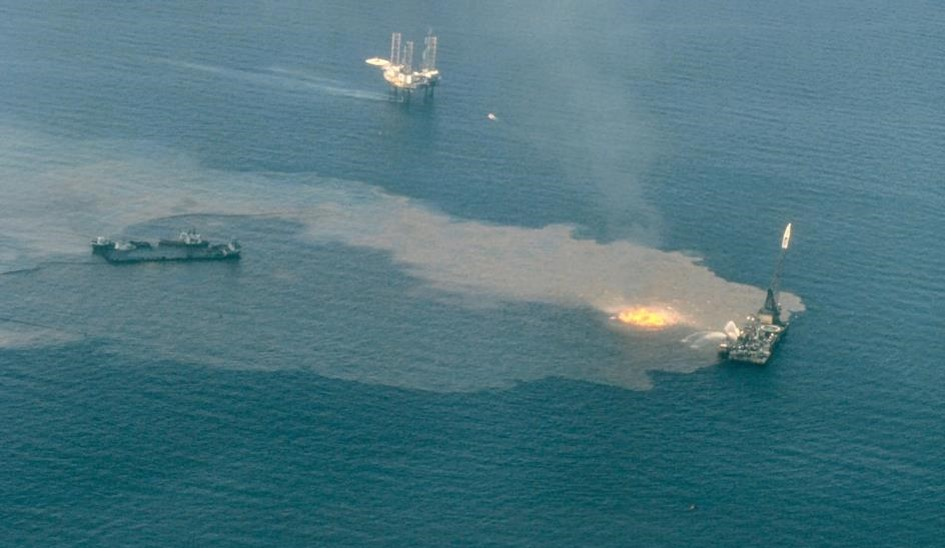
\includegraphics[scale=0.3]{img/section_01/explosion_ixtoc.jpg}
        \caption{Explosión del pozo Ixtoc I, Sonda de Campeche, 3 de junio de 1979}
        \label{fig:section_01_explosion_ixtoc}
    \end{figure}

    Estimación del derrame, 530,000 toneladas de crudo.
\end{frame}

\begin{frame}{Pozos perforados (2011 - 2013)}
    \begin{figure}
        \centering
        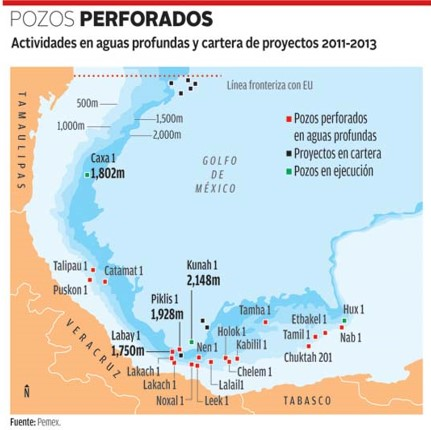
\includegraphics[scale=0.4]{img/section_01/pozos_perforados_2013.jpg}
        \caption{Actividades de exploración y perforación en 2013}
        \label{fig:section_01_pozos}
    \end{figure}
\end{frame}

\begin{frame}{Deep Water Horizon}
    \begin{figure}
        \centering
        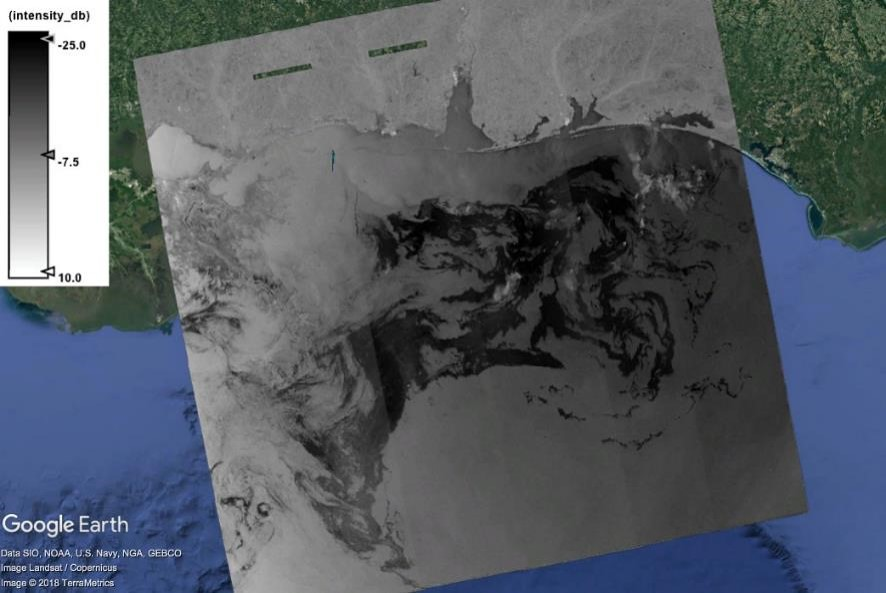
\includegraphics[scale=0.3]{img/section_01/deep-water-horizon.jpg}
        \caption{Extensión del derrame}
        \label{fig:section_01_deep_water_horizon}
    \end{figure}

    Estimación del derrame: 779,000 toneladas de crudo.
\end{frame}

\begin{frame}{Dinámica de la océano-petróleo}
    \begin{figure}
        \centering
        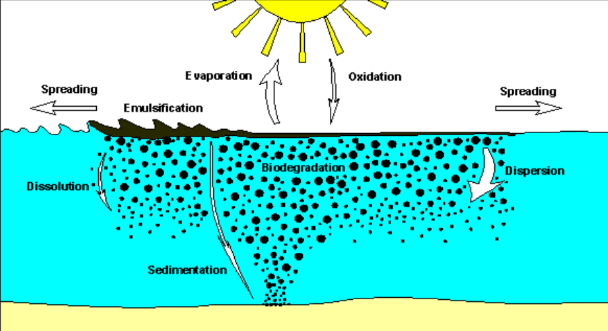
\includegraphics[scale=0.2]{img/section_01/dinamica-derrame.png}
        \caption{Dinámica de un derrame}
        \label{fig:section_01_dinamica_derrame}
    \end{figure}    
\end{frame}
